
%(BEGIN_QUESTION)
% Copyright 2005, Tony R. Kuphaldt, released under the Creative Commons Attribution License (v 1.0)
% This means you may do almost anything with this work of mine, so long as you give me proper credit

Determine the following parameters of these AC voltage waveforms, assuming a vertical sensitivity of 1 volt per division and a timebase of 2 milliseconds per division:

$$\includegraphics[width=15.5cm]{i00538x01.eps}$$

Also, determine which waveform is {\it leading} and which waveform is {\it lagging}.

\underbar{file i00538}
%(END_QUESTION)





%(BEGIN_ANSWER)

$V_{1}$ (peak) = 3 volts \hskip 100pt $V_{2}$ (peak) = 3.4 volts

\vskip 10pt

$f$ = 100 Hz \hskip 100pt $\theta$ = 72$^{o}$

\vskip 10pt

$V_1$ leads $V_2$ by +72$^{o}$.  $V_2$ lags $V_1$ by -72$^{o}$.

%(END_ANSWER)





%(BEGIN_NOTES)

It is important to have students explain {\it how} they solved for the phase shift, because many will have a tendency to follow a memorized equation, or worse yet follow {\it someone else's} memorized equation.  This is a really simple problem to solve, even if the only thing you remember about a sine wave is that a full cycle has 360 degrees of rotation.

%INDEX% Electricity review: phase shift measurement (dual-trace oscilloscope)

%(END_NOTES)


